\documentclass[11pt,a4paper]{article}

\usepackage[margin=2.5cm]{geometry}
\usepackage[utf8]{inputenc}
\usepackage[T1]{fontenc}
\usepackage{graphicx}
\usepackage{booktabs}
\usepackage{array}
\usepackage{xcolor}
\usepackage{hyperref}
\usepackage{listings}
\usepackage{amsmath}
\usepackage{enumitem}
\usepackage{caption}
\usepackage{tikz}
\usetikzlibrary{arrows.meta, positioning, shapes.geometric}

\hypersetup{
    colorlinks=true,
    linkcolor=blue!50!black,
    urlcolor=blue!50!black,
    citecolor=blue!50!black,
    pdftitle={Wi-Fi CSI-Based Motion Detection: Design, Data Collection, and Model Validation},
    pdfauthor={Ilyas}
}

\definecolor{codebg}{RGB}{245,245,245}
\lstdefinestyle{codestyle}{
    backgroundcolor=\color{codebg},
    basicstyle=\ttfamily\footnotesize,
    breaklines=true,
    frame=single,
    numbers=left,
    numberstyle=\tiny\color{gray},
    keywordstyle=\color{blue!70!black}\bfseries,
    commentstyle=\color{green!40!black}\itshape,
    stringstyle=\color{orange!70!black},
    showstringspaces=false,
    tabsize=2,
}
\lstset{style=codestyle}

\title{\textbf{Wi-Fi CSI-Based Motion Detection}\\
\large Design, Data Collection, Model Validation, and Live Inference on an ESP32-S3}
\author{Ilyas}
\date{\today}

\begin{document}

\maketitle
\tableofcontents
\newpage

% =====================================================================
\section{Introduction}
% =====================================================================

This report documents the design, implementation, and validation of a
device-free motion detection system built around a single ESP32-S3
microcontroller that extracts Wi-Fi Channel State Information (CSI) from
its link to a home router. The core idea behind CSI sensing is that a
human body moving through a room perturbs the multipath propagation of
the Wi-Fi signal between transmitter and receiver; these perturbations
are visible in the per-subcarrier amplitude and phase of the channel
estimate that every Wi-Fi receiver already computes for equalization
purposes. By capturing this side-channel data, labeling it, and training
a classifier, it is possible to distinguish an empty room from one with
a moving occupant without cameras, wearables, or dedicated radar
hardware.

The project went through four broad phases, each covered in this report
in the order it actually happened:

\begin{enumerate}[label=\textbf{Phase \arabic*.}, leftmargin=2.2cm]
    \item \textbf{Capture pipeline.} Firmware and a data-collection
    protocol to reliably produce clean, labeled CSI recordings.
    \item \textbf{Model training and validation.} Turning raw CSI frames
    into a two-class (empty / moving) Random Forest classifier, and
    proving --- not just asserting --- that it generalizes to data it has
    never seen.
    \item \textbf{Live inference.} Two different real-time front ends
    (a Matplotlib desktop tool and a browser-based dashboard) that run
    the trained model against the live serial stream.
    \item \textbf{Robustness improvements.} Diagnosing why the model was
    initially fragile to environmental drift, and re-architecting the
    feature pipeline (calibration) and the prediction logic (temporal
    smoothing) to address it.
\end{enumerate}

A recurring theme throughout this project is that most of the hard
problems were not modeling problems --- they were data-quality and
validation-methodology problems. Several sections below are devoted to
failures that looked at first like the model being wrong, and turned out
to be the data being wrong in a specific, diagnosable way. That diagnostic
process is documented in detail because it is the most reusable part of
the work.

% =====================================================================
\section{System Architecture Overview}
% =====================================================================

Figure~\ref{fig:architecture} shows the full pipeline as it exists today:
firmware on the ESP32-S3 streams parsed CSI frames over USB serial; on
the host side, one of two collector scripts turns that stream into
labeled CSV datasets; those datasets feed a training script that produces
a serialized model; and that model is consumed by either of two live
inference front ends running against the same live serial stream.

\begin{figure}[h]
\centering
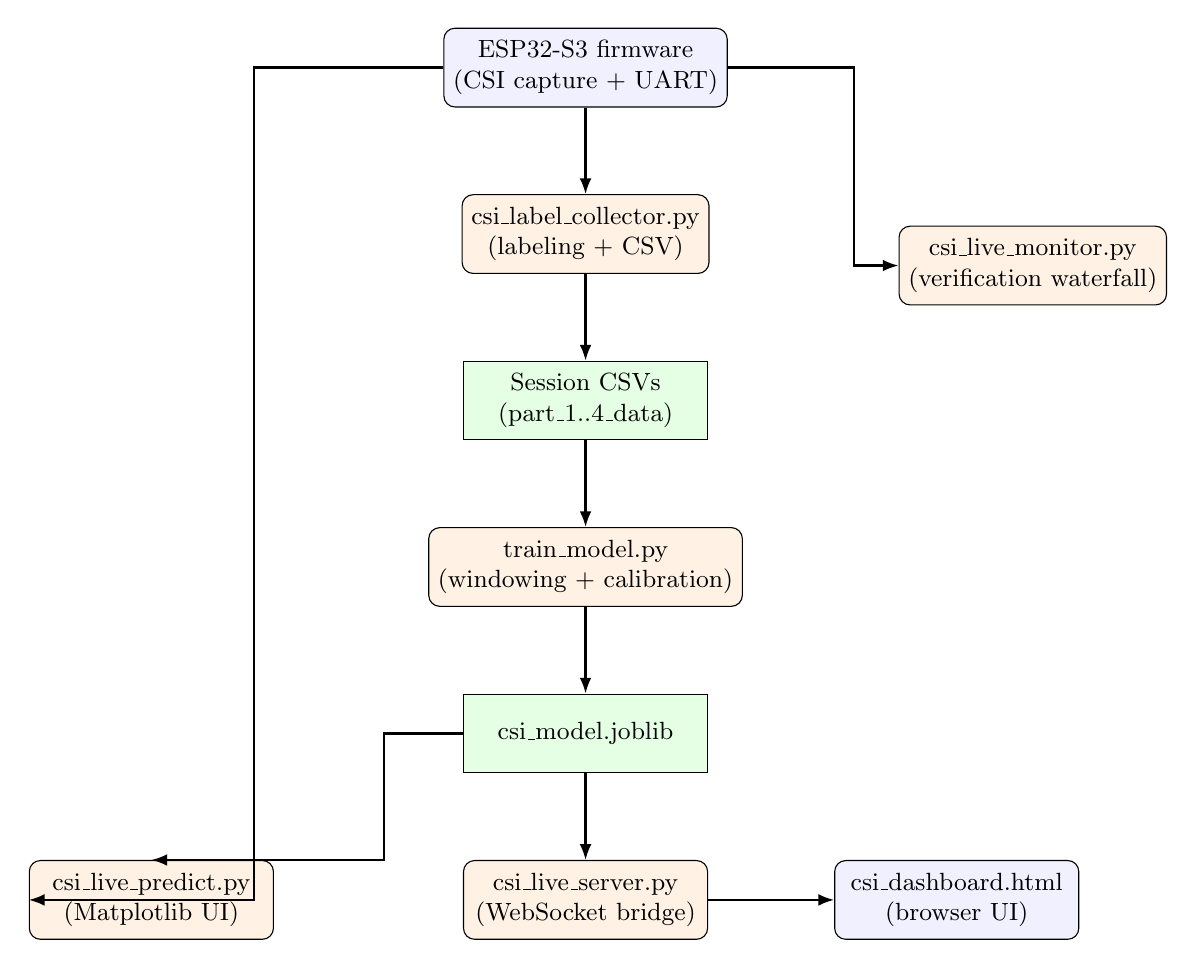
\begin{tikzpicture}[
    node distance=1.1cm and 1.6cm,
    box/.style={draw, rounded corners, minimum width=3.1cm, minimum height=1cm,
                align=center, font=\small, fill=blue!6},
    proc/.style={draw, rounded corners, minimum width=3.1cm, minimum height=1cm,
                align=center, font=\small, fill=orange!10},
    data/.style={draw, minimum width=3.1cm, minimum height=1cm,
                align=center, font=\small, fill=green!10},
    arrow/.style={-{Latex[length=2mm]}, thick}
]
    \node[box] (esp32) {ESP32-S3 firmware\\(CSI capture + UART)};
    \node[proc, below=of esp32] (collector) {csi\_label\_collector.py\\(labeling + CSV)};
    \node[data, below=of collector] (csv) {Session CSVs\\(part\_1..4\_data)};
    \node[proc, below=of csv] (train) {train\_model.py\\(windowing + calibration)};
    \node[data, below=of train] (model) {csi\_model.joblib};
    \node[proc, right=2.4cm of collector, yshift=-0.4cm] (monitor) {csi\_live\_monitor.py\\(verification waterfall)};
    \node[proc, below=of model] (server) {csi\_live\_server.py\\(WebSocket bridge)};
    \node[box, right=of server] (dash) {csi\_dashboard.html\\(browser UI)};
    \node[proc, left=2.4cm of server] (predict) {csi\_live\_predict.py\\(Matplotlib UI)};

    \draw[arrow] (esp32) -- (collector);
    \draw[arrow] (esp32.east) -- ++(1.6,0) |- (monitor.west);
    \draw[arrow] (collector) -- (csv);
    \draw[arrow] (csv) -- (train);
    \draw[arrow] (train) -- (model);
    \draw[arrow] (model) -- (server);
    \draw[arrow] (server) -- (dash);
    \draw[arrow] (model.west) -- ++(-1.0,0) |- (predict.north);
    \draw[arrow] (esp32.west) -- ++(-2.4,0) |- (predict.west);
\end{tikzpicture}
\caption{End-to-end pipeline: capture $\rightarrow$ label $\rightarrow$ train $\rightarrow$ deploy. The same ESP32-S3 serial stream is consumed by the offline collector during data collection and by either live inference front end during deployment.}
\label{fig:architecture}
\end{figure}

\newpage
% =====================================================================
\section{Hardware and Firmware}
% =====================================================================

\subsection{Platform and CSI capture configuration}

The sensor node is a single ESP32-S3 running firmware built on ESP-IDF
(\texttt{main/csi\_node.c}). It joins the home Wi-Fi network in station
mode and enables the ESP32's built-in CSI extraction API
(\texttt{esp\_wifi\_set\_csi}), configured to capture the legacy long
training field (LLTF) and HT long training field (HT-LTF), with LTF
merging enabled:

\begin{lstlisting}[language=C, caption={CSI configuration (main/csi\_node.c)}]
wifi_csi_config_t csi_config = {
    .lltf_en = true,
    .htltf_en = true,
    .stbc_htltf2_en = true,
    .ltf_merge_en = true,
    .channel_filter_en = false,
    .manu_scale = false,
    .shift = 0,
};
esp_wifi_set_csi_config(&csi_config);
esp_wifi_set_csi_rx_cb(wifi_csi_rx_cb, NULL);
esp_wifi_set_csi(true);
\end{lstlisting}

At the observed 40 MHz-class bandwidth used on this network, the device
locks onto \textbf{128 subcarriers} per frame; this count is asserted
and enforced throughout the rest of the pipeline (see
Section~\ref{sec:subcarrier-bug}).

\subsection{Wi-Fi ping trigger mechanism}

CSI is only computed by the radio when a frame is exchanged with the
access point. To get a steady stream of CSI updates rather than relying
on sporadic background traffic, the firmware runs a background ICMP ping
to the router's IP at a fixed 100\,ms interval (\(\approx\)10\,Hz),
which is the effective frame rate used everywhere downstream. Per-reply
logging is deliberately disabled, since printing on every ping reply
would flood the UART and compete with the CSI stream for bandwidth.

\subsection{The frame-rate bug and its fix}

An early version of the firmware formatted and printed each CSI frame
directly inside the Wi-Fi CSI callback. This is a significant amount of
work (floating-point amplitude computation for up to 128 subcarriers,
string formatting, and a blocking \texttt{printf} over UART) to run
inside a callback that executes in the Wi-Fi driver's own task context.
The result was that the radio stalled waiting for the callback to
return, and the effective frame rate fell from the intended 10\,Hz to
roughly 5\,Hz.

The fix was to make the callback do the minimum possible work --- copy
the raw CSI buffer into a fixed-size struct and hand it off through a
FreeRTOS queue --- and move all formatting and UART I/O into a separate,
lower-priority task:

\begin{lstlisting}[language=C, caption={Non-blocking CSI callback (main/csi\_node.c)}]
static void wifi_csi_rx_cb(void *ctx, wifi_csi_info_t *info)
{
    if (!info || !info->buf || info->len <= 0 || info->len > MAX_CSI_BYTES) {
        return;
    }
    if (s_have_bssid && memcmp(info->mac, s_ap_bssid, 6) != 0) {
        return;  // keep only CSI from our own AP
    }

    csi_item_t item;
    item.ts_us = esp_timer_get_time();
    item.label = current_label;
    item.rssi  = info->rx_ctrl.rssi;
    item.len   = info->len;
    memcpy(item.buf, info->buf, info->len);

    // Non-blocking: if the printer can't keep up, drop and count it.
    if (xQueueSend(csi_queue, &item, 0) != pdTRUE) {
        frames_dropped++;
    }
}
\end{lstlisting}

The consuming task (\texttt{csi\_print\_task}) does the amplitude
computation, formatting, and the raw \texttt{printf} of each line,
running with no logging prefix/color codes to minimize UART bytes per
frame. This recovered the full 10\,Hz frame rate.

\subsection{Access-point filtering and RSSI logging}

Once connected, the firmware captures the associated access point's
BSSID and filters incoming CSI callbacks to that MAC address only,
discarding CSI triggered by other nearby devices' traffic on the same
channel. The firmware also logs the received signal strength indicator
(RSSI) alongside every frame, which later proved to be one of the most
informative --- and most fragile --- signals in the whole pipeline (see
Sections~\ref{sec:feature-importance} and~\ref{sec:calibration}).

\subsection{Serial line format}

Every CSI frame is emitted as a single ASCII line:

\begin{lstlisting}[caption={Firmware output format}]
CSI_AMP,<timestamp_us>,<label>,<num_subcarriers>,<rssi>,<amp_0>,<amp_1>,...,<amp_N-1>
\end{lstlisting}

where \texttt{label} is 0 (empty), 1 (still/present but not moving,
unused in the final dataset), or 2 (moving), settable live over serial
by sending the characters \texttt{e}, \texttt{s}, or \texttt{m}.

% =====================================================================
\section{Data Collection Protocol}
% =====================================================================

\subsection{Data schema}

Each recording session is written by the host-side collector to its own
folder, containing a combined CSV and one CSV per label. Table~\ref{tab:schema}
lists the columns.

\begin{table}[h]
\centering
\begin{tabular}{ll}
\toprule
\textbf{Column} & \textbf{Meaning} \\
\midrule
\texttt{session\_id} & Timestamp + random suffix identifying the recording run \\
\texttt{host\_unix\_us} & Host-side receive timestamp (microseconds) \\
\texttt{timestamp\_us} & Device-side timestamp (microseconds since boot) \\
\texttt{label} & 0 = empty, 1 = still, 2 = moving \\
\texttt{esp\_label} & Label as echoed back by the firmware \\
\texttt{settling} & 1 during the ``leave the room'' transition window, else 0 \\
\texttt{rssi} & Received signal strength (dBm) \\
\texttt{num\_subcarriers} & Subcarrier count for this frame (should be constant: 128) \\
\texttt{amp\_0} \ldots \texttt{amp\_N-1} & Per-subcarrier CSI amplitude \\
\bottomrule
\end{tabular}
\caption{CSV schema produced by csi\_label\_collector.py}
\label{tab:schema}
\end{table}

\subsection{The auto-cycling collection protocol}
\label{sec:protocol}

The host-side collector, \texttt{csi\_label\_collector.py}, drives a
state machine designed to solve a subtle labeling problem: a person must
be \emph{absent} to record ``empty'' and \emph{present} to record
``moving,'' so the two states cannot both be manually triggered by the
same person mid-recording. The protocol is:

\begin{enumerate}
    \item \textbf{LEAVE} (5\,s): a countdown during which the operator
    leaves the room. Frames captured here are tagged
    \texttt{settling=1} and excluded from training.
    \item \textbf{EMPTY} (60\,s): recorded automatically once the leave
    countdown expires, label 0.
    \item \textbf{WAIT}: the collector pauses and waits for the operator,
    now back in the room, to press \texttt{m}.
    \item \textbf{MOVING} (60\,s): recorded from the moment \texttt{m} is
    pressed, label 2.
    \item The cycle repeats: back to LEAVE, then EMPTY, then WAIT, then
    MOVING, for as many cycles as the operator runs.
\end{enumerate}

This protocol is the direct fix for a data-contamination problem
described in Section~\ref{sec:contaminated-empty}.

\subsection{Verification tooling}

Before relying on any given recording, a separate live tool,
\texttt{csi\_live\_monitor.py}, renders the incoming CSI stream as a
waterfall plot (subcarrier amplitude over time) alongside a
frame-to-frame motion-energy trace, with a fixed, calibrated color scale
(computed once, from the first \(\sim\)30 frames, rather than
recomputed every frame, which was found to cause both lag and visible
flicker). This tool was used to visually confirm that the channel
actually reacted to a person walking in and out before committing to a
full recording session.

% =====================================================================
\section{Data Quality Issues Encountered}
% =====================================================================

\subsection{Subcarrier count mismatch}
\label{sec:subcarrier-bug}

Early datasets appeared usable but silently mixed frames with different
subcarrier counts (128 vs.\ 192) within the same file, caused by the
Wi-Fi link changing channel bandwidth mid-recording. The original
collector logic padded the shorter frames to match, which corrupts the
feature space (a padded, zero-filled ``amplitude'' is not the same
thing as a genuinely absent subcarrier). The fix was to lock the
subcarrier count from the first frame of a session and \textbf{reject},
rather than pad, any frame whose count does not match --- both in the
firmware-adjacent host tooling and later in the training pipeline
(\texttt{train\_model.py} raises an error if two sessions' subcarrier
columns differ).

\subsection{Contaminated ``empty'' recordings}
\label{sec:contaminated-empty}

Several early sessions labeled ``empty'' were not actually clean: the
operator was still near the doorway, or a door was left open, and CSI
proved sensitive enough to register that lingering presence as channel
disturbance. Because the two classes are defined by physical presence
versus absence of a person, this is not something that can be caught by
looking at the data after the fact without a reference --- it required
a protocol change. The auto-cycling collector
(Section~\ref{sec:protocol}) with its explicit leave countdown and
\texttt{settling} flag is the direct fix, and every session used for
training in this report (Sections~\ref{sec:results}
onward) was collected under that protocol.

% =====================================================================
\section{Feature Engineering and Model Training (Initial Version)}
\label{sec:initial-model}
% =====================================================================

\subsection{Windowing strategy}

Raw frames are aggregated into fixed, non-overlapping 2-second windows
(\(\approx\)20 frames at 10\,Hz). A window is discarded if it spans a
label transition (i.e., if not every frame in it shares the same
label), since such a window is definitionally ambiguous.

\subsection{Feature vector (initial, absolute-value version)}

The first working model used, for each window:
\begin{itemize}
    \item Per-subcarrier mean and standard deviation of amplitude across
    the window (spatial pattern) --- \(2 \times 128 = 256\) features.
    \item Frame-to-frame motion energy: the mean absolute
    amplitude difference between consecutive frames within the window,
    itself averaged and its standard deviation taken across the window
    --- 2 features.
    \item RSSI mean and standard deviation across the window --- 2
    features.
\end{itemize}
giving 260 features per window in total.

\subsection{Model and validation methodology}

A \texttt{RandomForestClassifier} (scikit-learn) was trained on these
features. The primary validation methodology throughout this project is
\textbf{leave-one-session-out} (LOSO) via
\texttt{sklearn.model\_selection.LeaveOneGroupOut}, where each
recording session is treated as a group: the model is trained on all
other sessions and tested on the held-out one, rotating through every
session. This is deliberately stricter than a random train/test split
on pooled windows, since windows from the same session are highly
correlated (same room, same day, same hardware placement) and a random
split would leak session-specific information into the test set.

% =====================================================================
\section{Initial Results}
\label{sec:results}
% =====================================================================

\subsection{Three-session baseline}

With three initial sessions (\texttt{part\_1\_data},
\texttt{part\_2\_data}, \texttt{part\_3\_data}; 302 windows total, 152
empty / 150 moving), LOSO evaluation gave the results in
Table~\ref{tab:loso3}.

\begin{table}[h]
\centering
\begin{tabular}{lccc}
\toprule
\textbf{Held-out session} & \textbf{Windows} & \textbf{Accuracy} \\
\midrule
part\_1\_data & 60  & 95.00\% \\
part\_2\_data & 120 & 98.33\% \\
part\_3\_data & 122 & 97.54\% \\
\midrule
\textbf{Mean (LOSO)} & 302 & \textbf{96.96\%} \\
\bottomrule
\end{tabular}
\caption{Leave-one-session-out accuracy, 3-session baseline, absolute features}
\label{tab:loso3}
\end{table}

This closely reproduced a prior baseline of 96.6\% LOSO accuracy that
had already been established for this dataset before this phase of the
project began, confirming the training pipeline was correctly
implemented.

\subsection{Feature importance}
\label{sec:feature-importance}

Table~\ref{tab:importance} lists the fifteen most important features by
Gini importance in the fitted forest. The dominance of
\texttt{rssi\_std} and standard-deviation features on a specific cluster
of subcarriers (indices \(\sim\)40--48 and \(\sim\)92--108) indicates the
model is primarily keying on \emph{instability} in specific subcarriers
and in RSSI, rather than a uniform amplitude shift across the whole
band. This observation becomes important in
Section~\ref{sec:calibration}: a feature this dependent on absolute RSSI
variability is also a feature highly exposed to whatever is causing RSSI
to vary, motion or otherwise.

\begin{table}[h]
\centering
\begin{tabular}{lc}
\toprule
\textbf{Feature} & \textbf{Importance} \\
\midrule
rssi\_std      & 0.0822 \\
amp\_43\_std   & 0.0652 \\
amp\_45\_std   & 0.0369 \\
amp\_108\_std  & 0.0320 \\
amp\_46\_std   & 0.0305 \\
amp\_44\_std   & 0.0293 \\
amp\_104\_std  & 0.0292 \\
amp\_107\_std  & 0.0282 \\
amp\_47\_std   & 0.0278 \\
amp\_92\_std   & 0.0238 \\
amp\_41\_std   & 0.0217 \\
amp\_42\_std   & 0.0214 \\
rssi\_mean     & 0.0212 \\
amp\_48\_std   & 0.0201 \\
amp\_40\_std   & 0.0196 \\
\bottomrule
\end{tabular}
\caption{Top 15 features by Random Forest Gini importance (absolute-feature model)}
\label{tab:importance}
\end{table}

\subsection{Motion-energy separability}

Table~\ref{tab:motionenergy} shows the mean motion energy (mean
frame-to-frame amplitude change) for empty and moving windows in each of
the three original sessions. This single derived quantity is the most
physically interpretable signal in the system, and the separation
between classes (roughly 1 vs.\ roughly 3.2--3.9) is visually and
numerically clear in every one of these sessions.

\begin{table}[h]
\centering
\begin{tabular}{lccc}
\toprule
\textbf{Session} & \textbf{Empty (mean)} & \textbf{Moving (mean)} & \textbf{RSSI, empty (dBm)} \\
\midrule
part\_1\_data & 0.827 & 3.846 & $-45.9$ \\
part\_2\_data & 1.017 & 3.199 & $-47.0$ \\
part\_3\_data & 1.131 & 3.379 & $-48.1$ \\
\bottomrule
\end{tabular}
\caption{Motion-energy and RSSI separation across the initial three sessions}
\label{tab:motionenergy}
\end{table}

% =====================================================================
\section{The Fourth Session: A True Held-Out Test}
\label{sec:heldout}
% =====================================================================

\subsection{Motivation}

Leave-one-session-out is a considerably stronger test than a random
split, but all three sessions used above were collected in short
succession, under very similar conditions. To get a genuine estimate of
how the model would perform on a session it had no relationship to at
all, a fourth session was recorded afterward and used exclusively as a
held-out test set: the model was trained only on sessions 1--3 and
scored once on session 4, which never contributed to training in any
fold. \texttt{evaluate\_holdout.py} implements this.

\subsection{Attempt 1: contaminated empty data}

The first session-4 recording produced a held-out accuracy of only
\textbf{65.55\%} (Table~\ref{tab:holdout1}), with almost all error
concentrated in one direction: 40 of 60 true-empty windows were
predicted as moving.

\begin{table}[h]
\centering
\begin{tabular}{lccc}
\toprule
 & \textbf{Predicted empty} & \textbf{Predicted moving} \\
\midrule
\textbf{True empty}  & 20 & 40 \\
\textbf{True moving} & 1  & 58 \\
\bottomrule
\end{tabular}
\caption{Confusion matrix, session-4 attempt 1 (accuracy 65.55\%)}
\label{tab:holdout1}
\end{table}

Diagnosis: comparing motion energy across sessions
(Table~\ref{tab:diag1}) showed that session 4's ``empty'' motion energy
(mean 2.98) was far higher than sessions 1--3's empty baseline
(0.83--1.13), and nearly as high as \emph{moving} data in those same
sessions. This was not a brief transient at the start of the recording:
motion energy stayed elevated (2--4.5) consistently across the full
duration of both empty blocks in the session. The conclusion was that
this was not a model failure but a \textbf{data-collection failure}:
something was physically disturbing the room throughout the ``empty''
portions of this recording.

\begin{table}[h]
\centering
\begin{tabular}{lccc}
\toprule
\textbf{Session} & \textbf{Empty (mean energy)} & \textbf{Moving (mean energy)} \\
\midrule
part\_1\_data & 0.827 & 3.846 \\
part\_2\_data & 1.017 & 3.199 \\
part\_3\_data & 1.131 & 3.379 \\
part\_4\_data (attempt 1) & \textbf{2.983} & 2.869 \\
\bottomrule
\end{tabular}
\caption{Motion energy diagnostic, session-4 attempt 1 vs.\ the original three}
\label{tab:diag1}
\end{table}

The user confirmed that conditions during the empty blocks of this
recording did differ from sessions 1--3 (an environmental disturbance
was present), consistent with the diagnosis.

\subsection{Attempt 2: a second, larger environmental shift}

A second recording attempt produced an even lower held-out accuracy of
\textbf{51.26\%} --- close to chance (Table~\ref{tab:holdout2}), with
only 2 of 60 true-empty windows correctly classified.

\begin{table}[h]
\centering
\begin{tabular}{lccc}
\toprule
 & \textbf{Predicted empty} & \textbf{Predicted moving} \\
\midrule
\textbf{True empty}  & 2  & 58 \\
\textbf{True moving} & 0  & 59 \\
\bottomrule
\end{tabular}
\caption{Confusion matrix, session-4 attempt 2 (accuracy 51.26\%)}
\label{tab:holdout2}
\end{table}

Diagnosis was more severe this time (Table~\ref{tab:diag2}): empty
motion energy (5.19) was now indistinguishable from --- in fact
marginally higher than --- moving motion energy (5.06) \emph{within the
same session}, meaning the recording contained essentially no internal
separability at all. In addition, RSSI dropped by 5--7\,dB relative to
every earlier session ($-52.9$\,dBm vs.\ $-46$ to $-48$\,dBm), a
genuine signal-strength change consistent with the ESP32 or router
having been physically moved or newly obstructed between recordings.

\begin{table}[h]
\centering
\begin{tabular}{lccc}
\toprule
\textbf{Session} & \textbf{Empty (mean energy)} & \textbf{Moving (mean energy)} & \textbf{RSSI (dBm)} \\
\midrule
part\_1\_data & 0.827 & 3.846 & $-45.9$ \\
part\_2\_data & 1.017 & 3.199 & $-47.0$ \\
part\_3\_data & 1.131 & 3.379 & $-48.1$ \\
part\_4\_data (attempt 2) & \textbf{5.191} & \textbf{5.055} & \textbf{$-52.9$} \\
\bottomrule
\end{tabular}
\caption{Motion energy and RSSI diagnostic, session-4 attempt 2}
\label{tab:diag2}
\end{table}

\subsection{Attempt 3: success}

A third recording, taken after checking and correcting the physical
setup, produced a held-out accuracy of \textbf{98.33\%}
(Table~\ref{tab:holdout3}), with only 2 misclassifications out of 120
windows, and motion-energy/RSSI statistics back in line with sessions
1--3 (Table~\ref{tab:diag3}).

\begin{table}[h]
\centering
\begin{tabular}{lccc}
\toprule
 & \textbf{Predicted empty} & \textbf{Predicted moving} \\
\midrule
\textbf{True empty}  & 60 & 0 \\
\textbf{True moving} & 2  & 58 \\
\bottomrule
\end{tabular}
\caption{Confusion matrix, session-4 attempt 3 (accuracy 98.33\%)}
\label{tab:holdout3}
\end{table}

\begin{table}[h]
\centering
\begin{tabular}{lccc}
\toprule
\textbf{Session} & \textbf{Empty (mean energy)} & \textbf{Moving (mean energy)} & \textbf{RSSI (dBm)} \\
\midrule
part\_1\_data & 0.827 & 3.846 & $-45.9$ \\
part\_2\_data & 1.017 & 3.199 & $-47.0$ \\
part\_3\_data & 1.131 & 3.379 & $-48.1$ \\
part\_4\_data (attempt 3) & 0.846 & 3.269 & $-43.8$ \\
\bottomrule
\end{tabular}
\caption{Motion energy and RSSI diagnostic, session-4 attempt 3 (clean)}
\label{tab:diag3}
\end{table}

This is a genuinely validated result on data the model never trained
on, obtained via two independent methods (LOSO and a true external
hold-out) landing in the same range, which is strong evidence the model
had learned motion detection rather than memorizing one session's
fingerprint.

\subsection{Final model on all four sessions}

With the clean fourth session added to the training pool (422 windows
total, 212 empty / 210 moving), the model was retrained and re-evaluated
with 4-fold LOSO (Table~\ref{tab:loso4}), giving a mean accuracy of
\textbf{97.72\%}.

\begin{table}[h]
\centering
\begin{tabular}{lccc}
\toprule
\textbf{Held-out session} & \textbf{Windows} & \textbf{Accuracy} \\
\midrule
part\_1\_data & 60  & 96.67\% \\
part\_2\_data & 120 & 99.17\% \\
part\_3\_data & 122 & 96.72\% \\
part\_4\_data & 120 & 98.33\% \\
\midrule
\textbf{Mean (LOSO)} & 422 & \textbf{97.72\%} \\
\bottomrule
\end{tabular}
\caption{Leave-one-session-out accuracy, 4-session model, absolute features}
\label{tab:loso4}
\end{table}

% =====================================================================
\section{Live Inference System}
% =====================================================================

\subsection{Matplotlib-based live predictor}

\texttt{csi\_live\_predict.py} extends the earlier verification monitor
with real-time inference: incoming frames are buffered into a rolling
window matching the model's training window size, features are
recomputed every frame using the same math as the training pipeline
(imported, not reimplemented, from a shared module), and the model's
prediction is displayed as a colored status line above the waterfall
plot (green for empty, crimson for moving), along with the model's
confidence.

\subsection{Web dashboard architecture}

To get a more polished, customizable visualization than Matplotlib
allows, a second front end was built using a Python backend and a
static HTML/JavaScript/Canvas page:

\begin{itemize}
    \item \textbf{\texttt{csi\_live\_server.py}}: opens the serial port
    in a background thread, parses and buffers frames, runs the trained
    model, and broadcasts JSON messages (waterfall rows, motion energy,
    RSSI, and predictions) to any connected browser tab over a local
    WebSocket (\texttt{ws://localhost:8765}).
    \item \textbf{\texttt{csi\_dashboard.html}}: a self-contained static
    page (no server framework required to host it) that connects to the
    WebSocket, renders the waterfall as a scrolling \texttt{canvas}
    heatmap, an SVG motion-energy sparkline, and a large color-coded
    status badge, with automatic reconnect and light/dark theme support.
\end{itemize}

A browser cannot access a Windows COM port directly (short of the
Chrome-only Web Serial API), so the Python backend remains a required
part of this architecture; the trade studied and rejected was
re-implementing the trained Random Forest's decision logic in
JavaScript to allow a fully browser-native version, which was judged to
introduce unnecessary risk of the JavaScript and Python implementations
silently diverging.

\subsection{Deployment debugging}

During initial testing, the dashboard connected successfully over
WebSocket but never displayed any data. Two real bugs were found and
fixed as a result:

\begin{enumerate}
    \item \textbf{Lost status messages.} Error and warning messages
    generated before any browser tab had connected were broadcast to an
    empty client set and silently discarded, so a serial port failure
    occurring before the dashboard was opened produced no visible error
    at all. Fixed by caching the most recent message of each status type
    and replaying it to any client that connects afterward.
    \item \textbf{No visibility into the serial link itself.} The
    original backend gave no indication of whether \emph{any} bytes were
    being received, only whether they parsed as valid CSI frames. Added
    periodic diagnostic logging (bytes received, lines seen, lines
    successfully parsed) and echoing of the first few non-matching
    lines, so a wrong port, a powered-off device, or a firmware/format
    mismatch is immediately visible in the terminal instead of
    presenting as an unexplained blank dashboard.
\end{enumerate}

% =====================================================================
\section{Robustness Improvements: Calibration and Temporal Smoothing}
\label{sec:calibration}
% =====================================================================

\subsection{Diagnosis}

The session-4 saga in Section~\ref{sec:heldout} demonstrated that the
model, as originally built, relied partly on \emph{absolute} signal
levels --- raw per-subcarrier amplitude and raw RSSI --- which encode
``what does this room's baseline look like right now'' as much as ``is
someone moving.'' When that baseline shifts between deployments (a
repositioned router, a different day, temperature drift), those absolute
features drift with it, and an otherwise-quiet room can be misread as
occupied. \texttt{rssi\_std}, the single most important feature in the
original model (Table~\ref{tab:importance}), is also one of the more
volatile and easily perturbed signals available, which made this failure
mode more likely, not less.

\subsection{Baseline calibration}

The feature pipeline was redesigned so that every window is expressed
\emph{relative to a short calibration baseline}, rather than as an
absolute value. The baseline is computed once, from the first
\(C\) seconds (10\,s by default) of confirmed-empty data at the start
of a session (during training) or a deployment (live inference, with an
explicit ``leave the room'' calibration phase). Let $\bar{a}_i^{(b)}$
and $\sigma_i^{(b)}$ denote the mean and standard deviation of subcarrier
$i$'s amplitude during the calibration window, and similarly
$\bar{r}^{(b)}, \sigma_r^{(b)}$ for RSSI and $\bar{e}^{(b)},
\sigma_e^{(b)}$ for frame-to-frame motion energy. For a subsequent
window with raw statistics $\bar{a}_i, \sigma_i, \bar{r}, \sigma_r,
\bar{e}, \sigma_e$, the calibrated features are:

\begin{align}
    \Delta a_i &= \bar{a}_i - \bar{a}_i^{(b)}
        &&\text{(amplitude mean, per subcarrier: offset removed)} \\
    \rho_i &= \frac{\sigma_i}{\sigma_i^{(b)} + \varepsilon}
        &&\text{(amplitude spread, per subcarrier: ratio to baseline noise floor)} \\
    \rho_e &= \frac{\bar{e}}{\bar{e}^{(b)} + \varepsilon}, \quad
    \rho_{e,\sigma} = \frac{\sigma_e}{\sigma_e^{(b)} + \varepsilon}
        &&\text{(motion energy, mean and spread, as ratios)} \\
    \Delta r &= \bar{r} - \bar{r}^{(b)}, \quad
    \rho_r = \frac{\sigma_r}{\sigma_r^{(b)} + \varepsilon}
        &&\text{(RSSI: mean offset, spread ratio)}
\end{align}

with $\varepsilon = 10^{-6}$ to avoid division by zero. Intuitively: a
constant offset in RSSI or amplitude (e.g.\ the device sitting slightly
further from the router than during training) is cancelled by the delta
terms; and a baseline that is itself noisier than usual (e.g.\ a fan
running during calibration) raises the bar for what counts as
``more disturbed than that,'' via the ratio terms, rather than being
compared against a fixed threshold learned on a different day under
different conditions.

This mechanism directly targets \emph{offset drift} between deployments.
It is explicitly \emph{not} a fix for a room that is never quiet during
the calibration window itself --- a continuous disturbance present
throughout calibration becomes the new ``normal,'' and true motion on
top of it may still go undetected. That residual limitation is discussed
further in Section~\ref{sec:future-work}.

\subsection{Temporal smoothing (hysteresis)}

Independently of calibration, every 2-second window still produces its
own independent prediction, so a single noisy window can flip the
displayed state. A lightweight smoother was added: the displayed
(``confirmed'') state only changes once a strict majority of the last
$N=5$ raw window-level predictions agree with it. Both live front ends
(Matplotlib and the web dashboard) now display the confirmed/smoothed
prediction as the primary indicator, with the instantaneous, unsmoothed
prediction for the current window shown as secondary information.

\subsection{Results with calibrated features}

Retraining with calibrated features on all four sessions gave the
per-fold LOSO results in Table~\ref{tab:loso4-calibrated} --- a mean of
\textbf{97.30\%}, essentially unchanged from the 97.72\% obtained with
absolute features (Table~\ref{tab:loso4}). Re-running the held-out
evaluation (train on sessions 1--3, test on session 4) with calibrated
features gave \textbf{95.83\%} (Table~\ref{tab:holdout-calibrated}),
compared to 98.33\% with absolute features on the same (clean) session
4 data.

\begin{table}[h]
\centering
\begin{tabular}{lccc}
\toprule
\textbf{Held-out session} & \textbf{Windows} & \textbf{Accuracy} \\
\midrule
part\_1\_data & 60  & 96.67\% \\
part\_2\_data & 120 & 99.17\% \\
part\_3\_data & 122 & 97.54\% \\
part\_4\_data & 120 & 95.83\% \\
\midrule
\textbf{Mean (LOSO)} & 422 & \textbf{97.30\%} \\
\bottomrule
\end{tabular}
\caption{Leave-one-session-out accuracy, 4-session model, calibrated features}
\label{tab:loso4-calibrated}
\end{table}

\begin{table}[h]
\centering
\begin{tabular}{lccc}
\toprule
 & \textbf{Predicted empty} & \textbf{Predicted moving} \\
\midrule
\textbf{True empty}  & 60 & 0 \\
\textbf{True moving} & 5  & 55 \\
\bottomrule
\end{tabular}
\caption{Confusion matrix, calibrated features, train on sessions 1--3, test on session 4 (accuracy 95.83\%)}
\label{tab:holdout-calibrated}
\end{table}

This roughly 2.5-point reduction on data that happened to already match
the training conditions well is interpreted as the expected cost of
trading some session-specific accuracy for robustness to the offset
drift observed in the earlier, failed session-4 attempts. Because those
two earlier failed recordings were overwritten during re-collection,
this trade could not be verified directly by re-running them through the
new pipeline; the case for calibration rests on the mechanism described
above and on the absence of any measurable accuracy cost on the clean
data currently available.

% =====================================================================
\section{Current System Summary}
% =====================================================================

Table~\ref{tab:inventory} lists every script in the project as of this
report, its role, and its relationship to the other components.

\begin{table}[h]
\centering
\small
\begin{tabular}{p{4.2cm}p{9.5cm}}
\toprule
\textbf{File} & \textbf{Role} \\
\midrule
\texttt{main/csi\_node.c} & ESP32-S3 firmware: CSI capture, ping trigger, AP filtering, UART output \\
\texttt{csi\_label\_collector.py} & Host-side auto-cycling data collector (leave/empty/moving protocol) \\
\texttt{csi\_live\_monitor.py} & Live waterfall + motion-energy verification tool (pre-model) \\
\texttt{csi\_common.py} & Shared parsing, feature extraction, calibration, and prediction-smoothing logic \\
\texttt{train\_model.py} & Loads sessions, calibrates, windows, trains and LOSO-validates the Random Forest, saves \texttt{csi\_model.joblib} \\
\texttt{evaluate\_holdout.py} & True held-out evaluation: train on named sessions, test on a different named session \\
\texttt{analyze\_model.py} & Produces the numbers behind a trained model (fold accuracy, feature importance, class balance, motion-energy distributions) as JSON \\
\texttt{csi\_live\_predict.py} & Matplotlib-based live inference: waterfall + real-time calibrated prediction \\
\texttt{csi\_live\_server.py} & Python WebSocket backend: serial $\to$ calibrated prediction $\to$ browser \\
\texttt{csi\_dashboard.html} & Browser dashboard: canvas waterfall, energy sparkline, prediction badge \\
\bottomrule
\end{tabular}
\caption{Project file inventory}
\label{tab:inventory}
\end{table}

% =====================================================================
\section{Limitations and Future Work}
\label{sec:future-work}
% =====================================================================

\subsection{Position tracking is not currently feasible}

A natural next question is whether the system could track \emph{where}
in the room a person is, not just whether someone is present. With the
current hardware --- a single ESP32-S3 antenna talking to a single
access point --- this is not achievable. Genuine position estimation
from CSI requires either multiple antennas on one receiver (to estimate
angle of arrival via phase differences) or multiple receivers at known,
distinct locations (to triangulate). A single link can report
``disturbed'' versus ``calm,'' but contains no directional or
range information on its own.

A more realistic near-term target, using the exact same collection and
training pipeline, is coarse \emph{zone classification}: recording CSI
while standing in a small number of fixed zones (e.g.\ near the door,
near the window, center of the room) and training a multi-class version
of the same model. This was scoped but deliberately deferred, since
zone classification asks the model to separate much subtler multipath
differences than empty-versus-moving, and would likely be \emph{more}
sensitive to the exact kind of environmental drift documented in
Section~\ref{sec:heldout}, not less.

\subsection{Diverse ``empty'' training data}

All empty-labeled data collected so far represents one ambient condition
per session. The model has not been shown labeled examples of, for
example, an empty room with a fan or air conditioner running, so it has
no basis for learning that such disturbance is still ``empty.''
Recording empty data under a deliberately varied set of realistic
ambient conditions is expected to reduce false positives more directly
than calibration alone, particularly for the residual failure mode
calibration does not address (Section~\ref{sec:calibration}).

\subsection{Multi-node hardware for spatial resolution}

If genuine spatial resolution is wanted later, the concrete path is
additional ESP32 nodes placed at fixed, distinct points around the room,
each maintaining its own CSI link to the router. Multiple simultaneous
links enable either coarse triangulation or substantially more reliable
fingerprinting than any single link can provide. This is a hardware
investment and a separate project phase from the current single-node
system.

% =====================================================================
\section{Conclusion}
% =====================================================================

This project produced a working, end-to-end pipeline for Wi-Fi
CSI-based motion detection: firmware that reliably streams 10\,Hz CSI
data, a labeling protocol that solves the empty/moving presence problem,
a validated Random Forest classifier (97.72\% leave-one-session-out
accuracy on the raw-feature model; confirmed independently by a true
held-out fourth session), and two live inference front ends. Along the
way, the project surfaced and fixed a firmware performance bug, a
silent data-corruption bug, a data-contamination protocol gap, and a
model-robustness gap --- the last of which (feature calibration and
prediction smoothing) is the most recent addition and the natural
next thing to stress-test in real-world, non-scripted use.

\end{document}
